\documentclass[../main.tex]{subfiles}

\begin{document}

\chapquote{Chess is the struggle against the error.}{Johannes Zukertort}
\chapter{Evaluation}
\label{chap:evaluation}
In \cref{chap:chess_recognition}, we evaluated the performance of each component in the chess recognition pipeline separately as well as the system as a whole, but that analysis was limited to the training and validation sets.
The test set remained untouched thus far for reasons concerning data leakage outlined in \cref{sec:split_dataset}.
Now we can evaluate the chess recognition system on the held-out test set because we have ensured that the models never before encountered this data.
\Cref{tbl:chess_recognition_trainvaltest_results} lists key evaluation metrics for the test set and contains the corresponding numbers from the other two datasets (as in \cref{tbl:chess_recognition_trainval_results}) for comparison.
\begin{table}
    \makebox[\textwidth][c]{
        \begin{tabular}{lrrr}
            \toprule
            metric & train & val & test \\
            \midrule
            mean number of incorrect squares per board           & 0.27    & 0.03     & 0.15 \\
            percentage of boards predicted with no mistakes      & 94.77\% & 97.95\%  & 93.86\% \\
            percentage of boards predicted with $\leq 1$ mistake & 99.14\% & 99.32\%  & 99.71\% \\
            per-board corner detection accuracy                  & 99.59\% & 100.00\% & 99.71\% \\
            per-square occupancy classification accuracy         & 99.81\% & 99.97\%  & 99.92\% \\
            per-square piece classification accuracy             & 99.99\% & 99.99\%  & 99.99\% \\
            \bottomrule
        \end{tabular}
    }
    \caption[Performance of the chess recognition system on the test dataset.]{Performance of the chess recognition system on the test dataset. The training and validation metrics as per \cref{tbl:chess_recognition_trainval_results} are included for comparison.}
    \label{tbl:chess_recognition_trainvaltest_results}
\end{table}
There is no indication of overfitting because there are only slight differences in the results of the train and test sets.
The two \glspl{cnn} perform on par or even better on the test set than the training set, and likewise does the corner detection algorithm.
However, these differences -- albeit suprising -- are negligible due to their insignificant magnitudes; in fact, the performance of on the validation set is even higher than on the test set.

The end-to-end per-board accuracy of our system on the unseen test set is 93.86\%, and if we allow just one mistake on the board, that accuracy increases to 99.71\%.
Comparing that first accuracy figure to the training set, we see a decrease of almost one percentage point. 
This might seem peculiar because the three main stages each performed better or on par with the scores of the training set.
However, if one takes into account that when permitting one mistake per board, the accuracy on the test set is actually higher than that of the training set, it becomes apparent that the the system had more incidences with two or more misclassified squares in the training set than the test set which is confirmed in \cref{fig:mistakes_frequency}.
\begin{figure}
    \makebox[\textwidth][c]{
        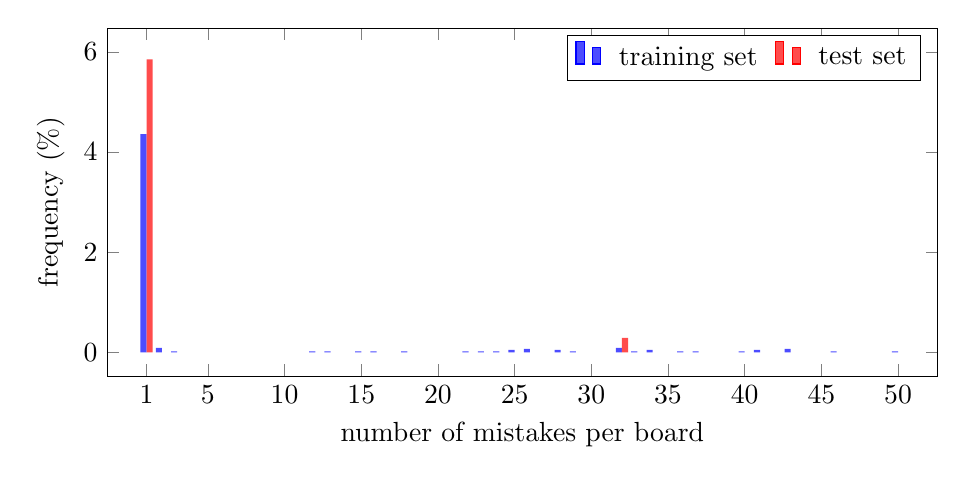
\begin{tikzpicture}
            \begin{axis}[
                width=\textwidth,
                height=6cm,
                ymin=0, ymax=6,
                ybar=0pt,
                bar width=.4,
                xlabel=number of mistakes per board,
                ylabel=frequency (\%),
                xmin=1,
                xtick={1,5,10,...,50},
                tick align=inside, 
                enlarge x limits={abs=.5cm},
                enlarge y limits={abs=.3cm},
                legend columns=2,
                legend style={
                    column sep=1ex
                }
            ]
                \addplot+[draw=none,fill=blue!70] coordinates {
                    ( 1, 4.36)
                    (32, 0.09)
                    ( 2, 0.09)
                    (26, 0.07)
                    (43, 0.07)
                    (34, 0.05)
                    (41, 0.05)
                    (28, 0.05)
                    (25, 0.05)
                    ( 3, 0.02)
                    (12, 0.02)
                    (16, 0.02)
                    (24, 0.02)
                    (15, 0.02)
                    (36, 0.02)
                    (40, 0.02)
                    (13, 0.02)
                    (46, 0.02)
                    (29, 0.02)
                    (23, 0.02)
                    (37, 0.02)
                    (50, 0.02)
                    (18, 0.02)
                    (22, 0.02)
                    (33, 0.02)
                };
                \addplot+[draw=none,fill=red!70] coordinates {
                    ( 1, 5.85)
                    (32, 0.29)
                };
                \legend{training set, test set}
            \end{axis}
        \end{tikzpicture}
    }
    \caption[Frequency of the number of mistakes per board on the training and test sets.]{Frequency of the number of mistakes per board on the training and test sets as a percentage of the total number of chessboards in the respective dataset. The frequency for zero mistakes is not displayed (94.77\% on the training set and 93.86\% on the test set as per \cref{tbl:chess_recognition_trainvaltest_results}) as that would make the $y$-axis too large. On the training set, 0.86\% of the boards were predicted with two or more errors, whereas on the test set that figure is 0.29\%. Incidences with more than three mistakes are usually due to the chessboard corner points being detected incorrectly.}
    \label{fig:mistakes_frequency}
\end{figure}
Furthermore, we find that the average number of misclassified squares is lies at 0.15 on the test set as compared to 0.27 on the training set.
The confusion matrix in \cref{tbl:confusion_matrix_test_set} facilitates a more detailed analysis of the mistakes.
\begin{table}
    \makebox[\textwidth][c]{
        \renewcommand{\arraystretch}{2.5}
        \begin{tabular}{c|c|*{13}{>{\centering\arraybackslash} m{.75cm}}|}
            \multicolumn{2}{c}{} & \multicolumn{13}{c}{predicted} \\
            \cline{3-15}
            \multicolumn{1}{c}{} 
            &
            & \raisebox{-.2cm}{\WhitePawnOnWhite} 
            & \raisebox{-.2cm}{\WhiteKnightOnWhite} 
            & \raisebox{-.2cm}{\WhiteBishopOnWhite} 
            & \raisebox{-.2cm}{\WhiteRookOnWhite} 
            & \raisebox{-.2cm}{\WhiteQueenOnWhite} 
            & \raisebox{-.2cm}{\WhiteKingOnWhite} 
            & \raisebox{-.2cm}{\BlackPawnOnWhite} 
            & \raisebox{-.2cm}{\BlackKnightOnWhite} 
            & \raisebox{-.2cm}{\BlackBishopOnWhite} 
            & \raisebox{-.2cm}{\BlackRookOnWhite} 
            & \raisebox{-.2cm}{\BlackQueenOnWhite} 
            & \raisebox{-.2cm}{\BlackKingOnWhite} 
            & \raisebox{-.2cm}{\phantom{\WhitePawnOnWhite}} \\
            \cline{2-15}
            \multirow{13}{*}{\rotatebox[origin=c]{90}{actual}}
            & \raisebox{-.2cm}{\WhitePawnOnWhite}                &  1894 &     0 &     0 &     1 &     0 &     0 &     0 &     0 &     0 &     0 &     0 &     0 &     1 \\
            & \raisebox{-.2cm}{\WhiteKnightOnWhite}              &     0 &   334 &     2 &     0 &     0 &     0 &     0 &     0 &     0 &     0 &     0 &     0 &     0 \\
            & \raisebox{-.2cm}{\WhiteBishopOnWhite}              &     0 &     0 &   392 &     0 &     0 &     0 &     0 &     0 &     0 &     0 &     0 &     0 &     0 \\
            & \raisebox{-.2cm}{\WhiteRookOnWhite}                &     0 &     0 &     0 &   520 &     0 &     0 &     0 &     0 &     0 &     0 &     0 &     0 &     0 \\
            & \raisebox{-.2cm}{\WhiteQueenOnWhite}               &     0 &     0 &     0 &     0 &   229 &     0 &     0 &     0 &     0 &     0 &     0 &     0 &     1 \\
            & \raisebox{-.2cm}{\WhiteKingOnWhite}                &     0 &     0 &     0 &     0 &     0 &   341 &     0 &     0 &     0 &     0 &     0 &     0 &     0 \\
            & \raisebox{-.2cm}{\BlackPawnOnWhite}                &     0 &     0 &     0 &     0 &     0 &     0 &  1878 &     0 &     0 &     0 &     0 &     0 &     2 \\
            & \raisebox{-.2cm}{\BlackKnightOnWhite}              &     0 &     0 &     0 &     0 &     0 &     0 &     0 &   355 &     0 &     0 &     0 &     0 &     0 \\
            & \raisebox{-.2cm}{\BlackBishopOnWhite}              &     0 &     0 &     0 &     0 &     0 &     0 &     0 &     0 &   378 &     0 &     0 &     0 &     0 \\
            & \raisebox{-.2cm}{\BlackRookOnWhite}                &     0 &     0 &     0 &     0 &     0 &     0 &     0 &     0 &     0 &   511 &     0 &     0 &     0 \\
            & \raisebox{-.2cm}{\BlackQueenOnWhite}               &     0 &     0 &     0 &     0 &     0 &     0 &     0 &     0 &     0 &     0 &   229 &     0 &     0 \\
            & \raisebox{-.2cm}{\BlackKingOnWhite}                &     0 &     0 &     0 &     0 &     0 &     0 &     0 &     0 &     0 &     0 &     0 &   341 &     0 \\
            & \raisebox{-.2cm}{\phantom{\WhitePawnOnWhite}}      &     3 &     0 &     0 &     0 &     0 &     0 &     9 &     1 &     0 &     0 &     0 &     0 & 14402 \\
            \cline{2-15}
        \end{tabular}
        \renewcommand{\arraystretch}{1}
    }
    \caption[Confusion matrix of the per-square predictions on the test set.]{Confusion matrix of the per-square predictions on the test set. The final row/column represents empty squares. Note that the results from chessboards whose corners were not detected correctly are ignored here.}
    \label{tbl:confusion_matrix_test_set}
\end{table}
The last row and column, representing the class `empty square', contain the greatest number of incorrect samples which is a result of the worse performance of the occupancy classifier compared to the piece classifier.
However, we must also take into account that the occupancy classifier has a more difficult task in this regard, since it must determine whether a square is empty even when it is occuluded by a piece in front of it.
The piece classifier which had an accuracy of 99.99\% makes only three errors: in two cases it confuses a knight with a bishop, and in one case a pawn with a rook.

The empirical results on the test set clearly demonstrate that the chess recognition system is highly accurate.
However, for such a system to be practically effective, it must also be able to perform an inference in a reasonable amount of time.
To test this, we record the inference time for each of the test set samples and compute the mean over all samples.
In fact, we can provide more granular insights by additionally recording the average time in executing each of the three stages in the pipeline.
We conduct this experiment twice on the dedicated lab machine: in the first trial, we use only the \gls{cpu} whereas we enable \gls{gpu} acceleration for the second run.
The machine is equipped with a quad-core 3.20GHz Intel Core i5-6500 \gls{cpu} and, as mentioned in \cref{chap:implementation}, a 6GB NVIDIA GeForce GTX 1060 \gls{gpu}.
\Cref{fig:chesscog_speed} shows that the system is around six times faster when utilising the \gls{gpu}.
\begin{figure}
    \centering
    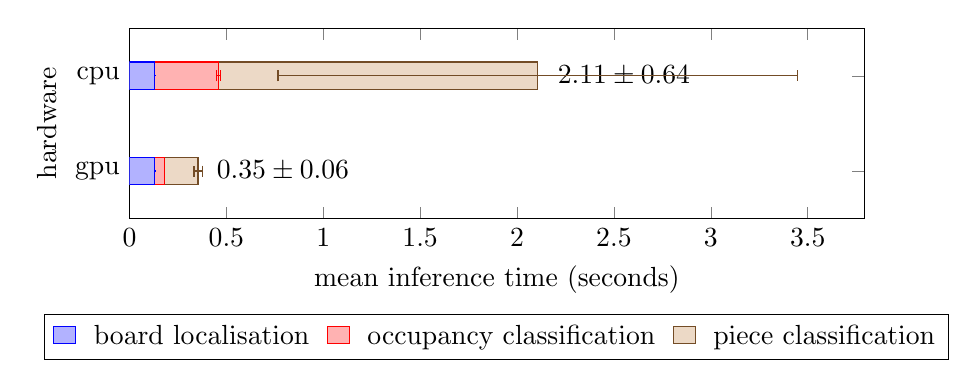
\begin{tikzpicture}
        \begin{axis}[
            width=.9\textwidth,
            height=4cm,
            xbar stacked,
            ylabel=hardware,
            xlabel=mean inference time (seconds),
            xmin=0,
            scaled ticks=false,
            stackedbar/.style = {
                xbar,
                error bars/.cd,
                x dir=both,
                x explicit relative
            },
            ytick={0,1},
            yticklabels={\acs{gpu},\acs{cpu}},
            % nodes near coords,
            y tick label style={align=center},
            enlarge y limits={abs=.5},
            legend columns=3,
            legend style={
                at={(0.5,-0.5)},
                anchor=north,
                column sep=1ex
            }
        ]
            \addplot+ [stackedbar] coordinates {
                (0.12935891456299406,0) +- (0.0069065603270334080,0)
                (0.12931111829404520,1) +- (0.0068571181376688630,0)
            };
            \addplot+ [stackedbar] coordinates {
                (0.05043862565584919,0) +- (0.0015867081771973946,0)
                (0.33029624063499774,1) +- (0.0219789229658819900,0)
            };
            \addplot+ [stackedbar] coordinates {
                (0.17394946628414532,0) +- (0.0593067253642730050,0)
                (1.64710188215145100,1) +- (0.6361857413955617000,0)
            };
            \node at (0.40, 0) [right] {$0.35 \pm 0.06$};
            \node at (2.16, 1) [right] {$2.11 \pm 0.64$};
            \legend{board localisation,occupancy classification,piece classification}
        \end{axis}
    \end{tikzpicture}
    \caption[Inference time benchmarks of the chess recognition pipeline on the test set.]{Inference time benchmarks of the chess recognition pipeline on the test set, averaged per sample. The error bars indicate the standard deviation and the mean total inference time is on the right of the bars. All benchmarks were carried out on the same machine (the Ubuntu lab machine described in \cref{chap:implementation}), although the data for the trial labelled \acs{cpu} was gathered without \acs{gpu} acceleration.}
    \label{fig:chesscog_speed}
\end{figure}
This is to be expected because the forward pass through the neural network executes many matrix operations that follow the \gls{simd} pattern and are thus well-suited for parallel computation on a \gls{gpu}.
Therefore, execution time of the occupancy and piece classifiers is significantly lower on the \gls{gpu}, whereas the board localisation (which runs on the \gls{cpu} regardless) takes a similar amount of time across both trials. 
Overall, the mean inference time is less than half a second on the \gls{gpu} and just over two seconds on the \gls{cpu}, although the latter measurement exhibits a significantly greater variance.
We conclude that the speed is sufficient for the intended practical purpose, and that the \gls{gpu}-accelerated pipeline would even be suited for real-time inference at 2-3 frames per second on just one \gls{gpu}.
Lastly, we see that the occupancy classifier needs just a fraction of the time required by the piece classifier.
This can be explained in the more complex architecture of the InceptionV3 network as opposed to the ResNet model and the greater input size which results in the number of parameter being twice as high in the piece classifier.

\section{Achievement of objectives}
All initial objectives described in the \gls{doer} document as well as the additional tertiary objective introduced in \cref{sec:objectives} have been successfully achieved in this project.
The following paragraphs provide evidence for the achievement of each objective in the order that they were specified in \cref{sec:objectives}.

\paragraph{Primary objectives}
The context survey of chess recognition systems in \cref{sec:context_survey_chess_recognition} is the outcome of objective \ref{obj:11} and is used to identify the limitations of current chess recognition systems to improve on them.
Next, the corner detection algorithm for localising chessboards (objective \ref{obj:12}) as detailed in \cref{sec:board_localisation} achieves an accuracy of 99.42\%, clearly highlighting its robustness.
Objective \ref{obj:13} concerns itself with the development of an algorithm for recognising chess pieces.
This is achieved in a two-stage process of occupancy classification (\cref{sec:occupancy_classification}) followed by piece classification (\cref{sec:piece_classification}) using \glspl{cnn}.
As a result, \cref{sec:preparing_results} explains how the entire pipeline is assembled, as required by objective \ref{obj:14}.
In accordance with the last primary objective \ref{obj:15}, the developed algorithms are each evaluated in isolation in \cref{chap:chess_recognition}, and then as a whole (\cref{sec:preparing_results} evaluates it on the validation set and at the beginning of this chapter, this is compared to the test set performance).

\paragraph{Secondary objectives}
\Cref{chap:data_synthesis} details the process of data synthesis, where the process of generating a large dataset of 4,800 labelled samples was automated using a 3D model in Blender, thus achieving objective \ref{obj:21}.
In line with objective \ref{obj:22}, \cref{sec:preparing_results} explains how the probability distribution over the squares is utilised to assemble an internal representation of the chess position which is then converted to \gls{fen} format.
The web \gls{api} for executing the inference pipeline as required by objective \ref{obj:23} is explained in \cref{sec:implementation_chessogapp} and available online at \url{https://www.chesscog.com/api/docs}.

\paragraph{Tertiary objectives}
Evidence for fulfilling objective \ref{obj:31} (implementing a proof-of-concept web app for chess position inference) lies in the fact that it is hosted online at \url{https://www.chesscog.com} and is explained in \cref{sec:implementation_chesscogapp,fig:webapp_overview}.
The \gls{fen} string is used to provide a link for opening the position in the board analysis tool on the popular chess website Lichess upon performing an inference.
Finally, the achievement of objective \ref{obj:32} is highlighted in \cref{chap:adapting}, where a process is devised for adapting the chess recognition system to new chess sets, using only two pictures of the board for training.
The success of this approach is reflected by the impressive results in \cref{tbl:transfer_learning_results}: based on just these two images, the system was able to correctly identify 88.89\% of the positions in the held-out test set, and all other positions had just one mistake.

Although not a formal objective, a deliberate emphasis was put on ensuring that the results claimed in this report are reproducible which even led to publishing a Python package (\texttt{recap}) on \gls{pypi} as a byproduct.
The datasets and trained models are made available for download, and all necessary code for training, inference, and evaluation is published on GitHub and supplied alongside the project submission.

\section{Critical appraisal}
\Cref{sec:context_survey_chess_recognition} surveys the state of the art in computer vision based approaches to chess recognition. 
Vision systems for chess robots or those designed for recording chess moves are inadequate for performing game state inference on a single image because these systems commonly rely on the difference between two images in order to determine the last move.
In the realm of single-image chess recognition systems (the type of system we aim to develop in this project), the context survey shows that systems exclusively employing traditional computer vision techniques are simply no match for approaches that effectively take advantage of deep learning.
However, systems with a poor piece classification performance might excel in their algorithm for board localisation.
Therefore, we will evaluate and compare our system to existing approaches across several different dimensions.
The context survey identifies the work of \textcite{mehta2020} as the current state of the art because it achieves the highest overall accuracy score and is one of the few works employing \glspl{cnn}, so in evaluating this project, a particular focus is put in the comparison to their system.

\paragraph{Datasets}
Many papers point out the lack of adequate datasets for chess recognition \cite{czyzewski2020,ding2016,mehta2020}.
Even though \citeauthor{czyzewski2018} published a dataset \cite{czyzewski2018} of difficult chessboard corners used to train their system\footnote{The dataset of \citeauthor{czyzewski2018} contains 9,664 black-and-white images of chessboard lattice points that are $21\times 21$ pixels in size and thus not sufficient to train a chess recognition system.} \cite{czyzewski2020}, large labelled datasets containing images of chess positions on a chessboard are not available as of now.
Yet it is well known that approaches based on deep learning tend to excel when supplied with large quantities of relevant data \cite{halevy2009}.
Most chess recognition systems to date use a dataset of chess photos the authors took themselves and had to annotate manually.
\Textcite{mehta2020}, whose dataset constitutes the largest in size, use a dataset of 2,622 occupied and vacant chessboard squares.
The dataset put forth in this project contains 4,888 samples of chess \emph{boards}, which means that there are 312,832 samples of chess \emph{squares}.
Manually creating a dataset of this size would have been infeasible; instead, we used a 3D model to render and automatically label the images.
For the benefit of future research in chess recognition systems and because our rendered dataset is two orders of magnitude larger than existing ones, we provide it publicly for download\footnote{As mentioned in \cref{chap:implementation}, the dataset is available at \url{https://tinyurl.com/chesscog-dataset}.}.

Nonetheless, the reader should note that the use of 3D models for data synthesis in the domain of chess recognition is not completely new:
\textcite{hou} use 3D chess set renderings to train their neural network, too, but their system uses just a simple non-convolutional \gls{ann} with only 1,000 squares for training and achieves an accuracy of only 72\%.
\textcite{wei2017} synthesise point cloud data for their volumetric \gls{cnn} directly from 3D chess models their approach works only if the chessboard was captured with a depth camera.

\paragraph{Board localisation}
Most chess robots circumvent the problem of board localisation by requiring manual calibration beforehand \cite{goncalves2005,sokic2008,khan2014}.
In fact, even some single-image approaches prompt the user to manually select the four corner points \cite{danner2015}, but that level of human intervention is not accaptable for the type of automatic chess recognition system this project aims to develop.

Some approaches to automatic chess grid detection utilise the Harris corner detector \cite{banerjee2012,hack2014}, but such algorithms fail when corners are occluded by pieces.
The most successful algorithms are based on line detection using the Hough transform \cite{tam2008,neufeld2010,danner2015,chen2016,kanchibail2016,xie2018a,chen2019} because that is more robust to occlusions.
As such, first step of our algorithm (\cref{sec:find_intersection_points}) is based on that idea: we detect lines by performing a Hough transform and then use a clustering algorithm to eliminate similar lines.
Then, we compute a perspective transformation of the grid lines that best matches the detected lines using a \gls{ransac}-based method.
Other techniques rely on the geometric nature of the chessboard as well \cite{tam2008,hack2014,danner2015,xie2018}, but rely on clustering algorithms instead of \gls{ransac}-based methods to eliminate outliers for computing the homography.
Although \textcite{hack2014} do employ a \gls{ransac}-like algorithm, they use it just for distinguishing between horizontal and vertical lines, and directly for fitting the homography as explained in \cref{sec:find_optimal_homography}.
Finally, we infer missing lines by computing horizontal and vertical gradients on the transformed image (\cref{sec:infer_missing_lines}), a novel technique that is not employed by the other recognition systems.
\Textcite{czyzewski2020} achieves the highest reported\footnote{\Citeauthor{mehta2020} do not separately report the board localisation accuracy.} board localisation accuracy of 95\%.
Our system outperforms this by more than four percentage points, achieving 99.71\% on the test set.

\paragraph{Piece classification}
Our approach to piece classification is a two-step process:
\cite{mehta2020} reports accuracy only on a per-square basis
\footnote{
    \Cref{tbl:chess_recognition_trainvaltest_results} does not explicitly report the per-square accuracy of the whole system.
    However, the mean number of incorrect squares per board was 0.15, so the per-square accuracy is $1-\sfrac{0.15}{64}=99.72\%$.
}

\paragraph{Adapting to different chess sets}

\ifSubfilesClassLoaded{%
\printglossary[type=\acronymtype]%
\printbibliography%
}{}%

\end{document}